% Preamble
%\documentclass[xetex,mathserif,serif]{beamer}
\documentclass{beamer}

% Packages
\usepackage[spanish]{babel}
\selectlanguage{spanish}
\usepackage[utf8]{inputenc} % For spanish (and international) letters like acents.
\usepackage{hyperref} % To create hyperlinks within the document.
\usepackage{graphicx} % To include graphics (pictures, images)
\usepackage{float} % For the use of the parameter "H" in command "\begin{figure}[H]" (i.e. exact position of image in text)
\usepackage{verbatim} % For long comments
\usepackage{tikz} % For include Dia diagrams in .tex format

\graphicspath{{../Diagramas/}} % Path of the folder containing the images

\title[Sistema web metaDOC]
{Sistema web para la catalogación y acceso a la información de una colección de documentales}
\subtitle{}
\author{Rodrigo~Colín\inst{1}, Sergio~Amaro\inst{2}}
\institute
{
	\inst{1}
	Laboratorio Audiovisual de Investigación Social\\
	Instituto Mora
	\and
	\inst{2}
	Facultad de Ciencias\\
	Universidad Nacional Autónoma de México
}
\date{JIAI 2016, 8 de junio de 2016}
%\subject{Catalogación de Colección de Documentales}


\AtBeginSection[]
{
  \begin{frame}
    \frametitle{Tabla de contenidos}
    \tableofcontents[currentsection]
  \end{frame}
}
\begin{comment}
\AtBeginSubsection[]
{
  \begin{frame}
    \frametitle{Tabla de contenidos}
    \tableofcontents[currentsection,currentsubsection]
  \end{frame}
}
\end{comment}

% Style and theme
\usetheme{PaloAlto}
%\usecolortheme{orchid} %crane,dolphin,lily

% Document environment
\begin{document}

\frame{\titlepage} % Página inicial

\section{Colección documental}
\begin{frame}
	\frametitle{El LAIS}
	\framesubtitle{Acerca del laboratorio}
	
	El Laboratorio Audiovisual de Investigación Social (LAIS) es un espacio colectivo e interdisciplinario dedicado a la \textbf{investigación social} con imágenes y que ha construido un acervo documental que se origina en 1993.

	Para el LAIS es una tarea prioritaria el resguardo y documentación de materiales audiovisuales para quienes recurrimos a ellos con fines de investigación.
	
\end{frame}


\begin{frame}
	\frametitle{El LAIS}
	\framesubtitle{Colección audiovisuales}
	
	La colección de materiales audiovisuales consta de tres series:
	\begin{enumerate}
		\item Documentales en video
		\item Registros en video
		\item Material de archivo
	\end{enumerate} \pause
	
	Nuestro énfasis está en la serie de \textbf{Documentales en video}. Constituida por \textbf{cine documental} recopilado desde los antecedentes del LAIS en diversos videoforos y cursos.
	
\end{frame}


\section{Catalogación}
\begin{frame}
	\frametitle{Catalogación}
	\framesubtitle{Acerca de ISAD(G)}
	
	¿Para qué catalogar?: Para preservar y \textbf{utilizar}.
	
	Por lo tanto se emplea la norma \textbf{ISAD(G)} (\textit{General International Standard Archival Description}) como base para la catalogación, ya que es el estándar para registrar documentos de archivo.
\end{frame}


\begin{frame}
	\frametitle{Manual de Catalogación}
	\framesubtitle{Para el acervo documental en video del LAIS}
	
	Para el caso particular de la colección de documentales en video del LAIS, la norma ISAD(G) es adaptada y el resultado es el ``\textbf{Manual de Catalogación para Documentales en Video del LAIS}'' que contempla las siguientes áreas de descripción:
	
	\begin{enumerate}
		\item Identificación
		\item Contexto
		\item Contenido y estructura
		\item Condiciones de acceso y uso
		\item Documentación asociada
		\item Notas
		\item Control de la descripción
	\end{enumerate}
\end{frame}


\section{Situación y propuesta}
\begin{frame}
	\frametitle{Situación y Propuesta}
	\framesubtitle{Para poner en acceso la ficha de los documentales}
	
	\begin{block}{Situación}
	Las fichas de documentación se tenían registradas en varias \textbf{hojas de cálculo} de Excel.
	\end{block} \pause
	
	\begin{block}{Propuesta}
	Hacer un \textbf{sistema} que administre y ponga en \textbf{acceso} estas fichas documentales. Se requiere crear una base de datos y una interfaz visual en donde lo usuarios puedan consultar dicha información.
	\end{block}
	
\end{frame}


\begin{frame}
	\frametitle{Propuesta de sistema}
	\framesubtitle{Esquema general}
	\begin{figure}[H]
		\centering
		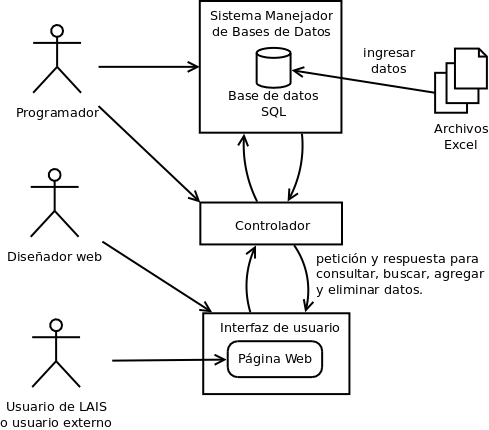
\includegraphics[width=0.7\textwidth]{EsquemaGeneral.png}
		\caption{Esquema general del sistema (aplicación web) para la catalogación y acceso de la colección de documentales del LAIS}
		\label{fig:esquema_general}
	\end{figure}
\end{frame}


\begin{frame}
	\frametitle{Requisitos a cumplir}
	
	\begin{itemize}
		\item Crear y poblar la base de datos con la información existente.
		\item Permitir agregar, modificar y eliminar fichas de documentación.
		\item Crear un sitio web (interfaz) eficiente y simple de usar.
		\item Control de quién puede realizar cambios en el sistema.
		\item Realizar búsquedas de contenido.
	\end{itemize}
\end{frame}


\section{Implementación}
\begin{frame}
	\frametitle{El sitio metaDOC}
	\framesubtitle{Documental e investigación}
	Tras meses de trabajo, el resultado es un sitio web llamado \textbf{metaDOC} que cumple con las necesidades originales de resguardo de información mediante bases de datos y puesta en acceso con apoyo de internet.
\end{frame}


\begin{frame}
	\frametitle{Demostración}
	\framesubtitle{Versión preliminar}
	
	\begin{figure}[H]
		\centering
		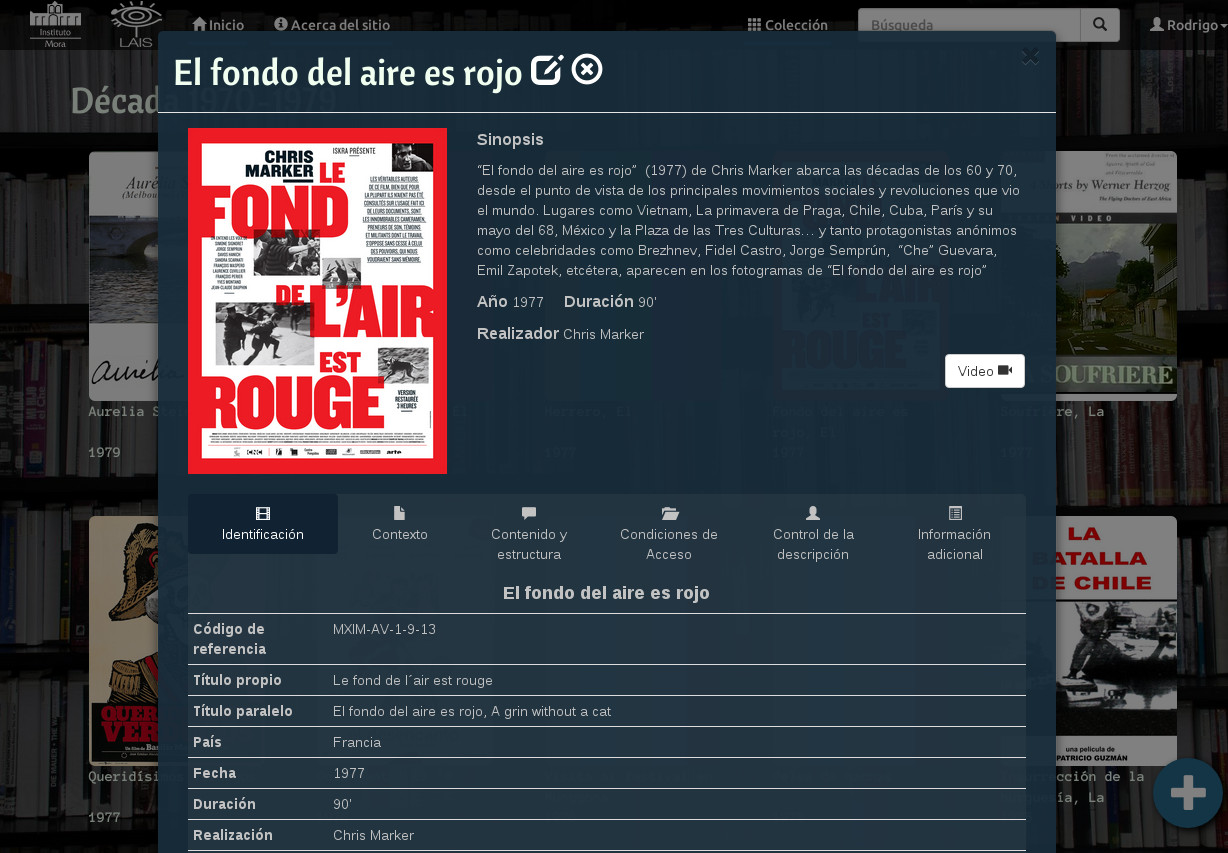
\includegraphics[width=0.7\textwidth]{Sistema01.jpg}
		\caption{Captura de pantalla del sistema metaDOC, muestra la ficha de un documental. (\url{lais-interno.mora.edu.mx/beta/public/})}
		\label{fig:sistema01}
	\end{figure}
\end{frame}


\section{Conclusión}
\begin{frame}
	\frametitle{Conclusiones}
	\begin{itemize}
		\item Mediante este sistema, incentivar la \textbf{consulta} de la ficha y los contenidos de los materiales audiovisuales para todas las personas interesadas.\pause
		\item Permitió una revisión y \textbf{reflexión} acerca de la forma de documentar.\pause
		\item El uso de \textbf{software libre} para dar soluciones a problemas de reguardo y documentación de materiales audiovisual.\pause
		\item La escalabilidad y futuro \textbf{desarrollo} del sistema.
	\end{itemize}
\end{frame}

\begin{frame}
	\begin{center}
		De parte de todos los integrantes del Laboratorio Audiovisual de Investigación Social (LAIS)
		
		¡GRACIAS!
		
		%logo del LAIS
		%
\includegraphics{scientistapprovedfutura.png}
	\end{center}
\end{frame}

\end{document}